\documentclass{article}
\usepackage{../math_template}

\author{Jonathan Kasongo}
\title{Canadian Junior Math Olympiad 2024 --- P1/5}

\begin{document}
\maketitle

\begin{problem}{Canadian Junior Math Olympiad 2024 --- P1/5}
Centuries ago, the pirate Captain Blackboard buried a vast amount of treasure in a
single cell of a $2 \times 4$ grid-structured island. You and your crew have reached the island
and have brought special treasure detectors to find the cell with the treasure. For each
detector, you can set it up to scan a specific subgrid $[a, b] \times [c, d]$ with $1 \leq a \leq b \leq 2$
and $1 \leq c \leq d \leq 4$. Running the detector will tell you whether the treasure is in the
region or not, though it cannot say where in the region the treasure was detected. You
plan on setting up $Q$ detectors, which may only be run simultaneously after all $Q$
detectors are ready. What is the minimum $Q$ required to guarantee your crew can
determine the location of Blackboard’s legendary treasure?
\end{problem}

\begin{solution}{Solution}
We claim that the minimum $Q$ is 3. First we show a construction that
works with $Q=3$, then we show that it is impossible to have smaller $Q$.\\

Observe the following diagram, \vspace{0.1cm}

\begin{center}
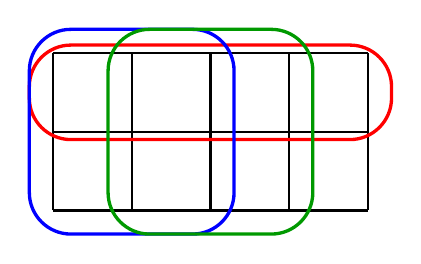
\begin{tikzpicture}[scale=1]
  % Grid: 4 columns (x: 0..4), 2 rows (y: 0..2)
  \draw[step=1cm, line width=0.8pt] (0,0) grid (4,2);

  % Red rounded rectangle: top row
  \draw[red, very thick, rounded corners=15pt]
    (-0.3,0.9) rectangle (4.3,2.1);

  % Blue rounded rectangle: leftmost 2x2 subgrid
  \draw[blue, very thick, rounded corners=15pt]
    (-0.3,-0.3) rectangle (2.3,2.3);

  % Green rounded rectangle: next 2x2 subgrid (one square to the right)
  \draw[green!60!black, very thick, rounded corners=15pt]
    (0.7,-0.3) rectangle (3.3,2.3);
\end{tikzpicture}
\end{center}

setting up the detectors like so will guarentee that the crew is able
to locate the treasure, since each square will alert a distinct set of
detectors (this can easily be checked by hand). \\

Note that the only way to guarentee that the crew can determine
the location of the legendary treasure is to have each square alert a
distinct set of treasure detectors, because if we don't do this then there
will be a set of squares that alert the same set of detectors and then the
crew won't be able to guarentee knowledge of the location of the treasure.
If the crew uses $Q$ treasure detectors then there exists

$$
\sum_{r=0}^Q \binom{Q}{r} = (1 + 1)^Q = 2^Q
$$

different sets of treasure detectors that could be alerted. Since
$2^1 < 2^2 < 2^3 = 8$, the minimum value of $Q$ is indeed 3. $\blacksquare$
\\

\textit{Remark: The intuition can come from computer science. It is well
known that, given a sorted list $L$ it is possible to
search the list in $\mathcal{O}(\log_2 n)$ time. Since there are
$8 = 2^3$ cells in this case, it is natural to guess that a possible
answer may be $\min Q = 3$.}
\end{solution}

\end{document}
